% !TEX root = ./informe.tex

\section{Problema 3}

\subsection{Explicación}

En una provincia, hay ciudades conectadas por rutas bidireccionales. No todas estan conectadas. Se quiere que exista una única forma de llegar de una ciudad a cualquier otra. Para logar esto, se pueden \textbf{destruir} rutas existentes o \textbf{construir} nuevas rutas. La construcción y destrucción de cada ruta tiene un costo asociado, por lo que se quiere además minimizar el costo. \\

Para resolver el problema podemos pensarlo como un problema de grafos. La provincia es un \textit{grafo}, donde cada ciudad es un \textit{nodo} y las rutas son \textit{aristas}.  \\

Si consideramos al grafo como el completo de \textit{n} nodos (donde \textit{n} es la cantidad de ciudades). Que exista una y solo una ruta para llegar de una ciudad a cualquier otra, significa que tenemos que lograr que las rutas existentes formen un árbol (que incluya a todos los nodos).  \\

Como podemos construir rutas nuevas y destruit las existentes, podríamos en principio quedarnos con cualquier árbol generador del grafo completo de \textit{n} nodos. Esto hace que las rutas elegidas cumplan la condición de conexiones. Restaría considerar que las rutas elegidas tienen además que tener el mínimo costo posible. \\

Las observaciones claves son las siguientes: \\
- Si se tiene que elegir entre construir dos rutas que no existen, lo mejor es construir la mas barata. \\
- Si se tiene que elegir entre destruir dos ya existentes, es mejor quedarse con la mas cara de destruir. \\
- Si se tiene que elegir entre mantener una ruta existente o destruirla y construir otra, es mas barato manterla. Mantener una ruta cuesta 0, mientras que destruirla y construir otra tiene costo. \\

Teniendo esto en cuenta, podemos armar nuestro grafo de la siguiente manera: \\

Tomamos un grafo completo de \textit{n} nodos. Las rutas que \textbf{no} existian las colocamos con su costo de construcción. Las rutas que \textbf{sí} existían las colocammos con el peso \textbf{negativo} de su destrucción. ¿Por qué el negativo? Al tratar de elegir los menores costos, se prioriza elegir una ya construida a una que no lo está, y entre dos construidas prioriza aquella que cuesta mas destruir. \\

La solución final es el Arbol Generador Mínimo de este grafo. \\


\subsection{Correctitud}
El problema habla de ciudades conectadas por rutas con ciertos costos asociados, lo cual vamos a modelar con grafos y funciones de pesos sobre aristas. Los grafos vendrán a ser subgrafos de un grafo completo de $n$ aristas, donde cada subgrafo representa una configuración distinta de rutas finales. Además, el enunciado nos pide que sean árboles, pues requiere que haya un sólo camino entre todo par de ciudades. Faltaría definir correctamente la función de peso, y minimizarla sobre los árboles candidatos a soluciones. \\

Definir la función de peso no es trivial: ejes destruidos aportan al costo de grafos cuando no pertenecen a ellos. La función que vamos a considerar es la siguiente: a las rutas inexistentes les vamos a asignar su costo de construcción, mientras que a las rutas ya construidas tendran como peso el opuesto de su costo de destrucción. El costo real de un posible grafo solución será entonces la suma de todos los costos de destrucción de la \textbf{entrada} menos el peso del grafo. \\

¿Por qué pesos negativos? Observemos por casos qué ocurre con un eje existente. Si lo destruimos, aporta su costo de destrucción cuando sumamos el de todos las rutas ya construidas. Si por el contrario lo incluimos como solución, su aporte se cancela con el peso negativo del eje, con lo cual termina con costo neto 0. Esto es lo que estabamos buscando modelar. \\

Resta ver cómo minimizar el costo que definimos. Observemos que para una entrada fija, la suma de los costos de destrucción es constante, con lo cual el costo total de un grafo es su peso más una constante, con lo cual nos basta con minimizar la función de peso. Además, estos grafos son árboles subgrafos de nuestro grafo completo de entrada. Por todo esto, el problema termina reduciéndose a encontrar el arbol generador mínimo de dicho grafo completo con nuestra función de peso.

\subsection{Pseudocódigo}

Vamos a utilizar como entrada en nuestro algoritmo las siguientes variables:
\begin{itemize}
	\item $n$: La cantidad de ciudades
	\item $existe$: El grafo de entrada representado con matriz de adyacencia.
	\item $costo$: La matriz con los costos de construcci\'on o destrucci\'on.
\end{itemize}

\begin{algorithm}[H]
% \label{ej3}         % and a label for \ref{} commands later in the document
\begin{algorithmic}
\Function{Resolver}{}    \Comment{$\mathbf{\mathcal{O}(n^2)}$}
	\State $costoInicialDestruirTodo \gets$ NegativizarCostoConstruidas()    \Comment{$\mathcal{O}(n^2)$}
	\State $arbol \gets$ PrimNaive()    \Comment{$\mathcal{O}(n^2)$}
	\State \Return ObtenerCostoTotal($arbol, costoInicialDestruirTodo$)    \Comment{$\mathcal{O}(n)$}
\EndFunction

\end{algorithmic}
\end{algorithm}

\begin{algorithm}[H]
\begin{algorithmic}

\Function{NegativizarCostoConstruidas}{}    \Comment{$\mathbf{\mathcal{O}(n^2)}$}
	\State $costoInicialDestruirTodo \gets 0$    \Comment{$\mathcal{O}(1)$}
	\For{$i \in [0..n)$}    \Comment{$\mathcal{O}(n)$}
		\For{$j \in [1..n]$}    \Comment{$\mathcal{O}(n)$}
			\If{$existe[i][j]$}    \Comment{$\mathcal{O}(1)$}
				\State $costoInicialDestruirTodo \gets costoInicialDestruirTodo + costo[i][j]$    \Comment{$\mathcal{O}(1)$}
				\State $costo[i][j] \gets -costo[i][j]$    \Comment{$\mathcal{O}(1)$}
				\State $costo[j][i] \gets -costo[j][i]$    \Comment{$\mathcal{O}(1)$}
			\EndIf
		\EndFor
	\EndFor
	\State \Return $costoInicialDestruirTodo$    \Comment{$\mathcal{O}(1)$}
\EndFunction

\end{algorithmic}
\end{algorithm}


\begin{algorithm}[H]
\begin{algorithmic}

\Function{ObtenerCostoTotal}{$arbol: Int[], costoInicialDestruirTodo: Int$}    \Comment{$\mathbf{\mathcal{O}(n)}$}
	\State $costoTotal \gets costoInicialDestruirTodo$    \Comment{$\mathcal{O}(1)$}
	\For{$i \in [2..n]$}    \Comment{$\mathcal{O}(n)$}
		\State $j \gets arbol[i]$    \Comment{$\mathcal{O}(1)$}
		\State $costoTotal \gets costoTotal + costo[i][j]$    \Comment{$\mathcal{O}(1)$}
	\EndFor
	\State \Return $costoTotal$    \Comment{$\mathcal{O}(1)$}
\EndFunction
\end{algorithmic}
\end{algorithm}


\begin{algorithm}[H]
\begin{algorithmic}
\Function{PrimNaive}{}    \Comment{$\mathbf{\mathcal{O}(n^2)}$}
	\State $visitado \gets Bool[n+1]$    \Comment{$\mathcal{O}(1)$}
	\State $dist \gets Int[n+1]$    \Comment{$\mathcal{O}(1)$}
	\State $padre \gets Int[n+1]$    \Comment{$\mathcal{O}(1)$} \\

	\State ($\forall$ i $\in$ [1..n]) $visitado[i] \gets$ False    \Comment{$\mathcal{O}(n)$}
	\State ($\forall$ i $\in$ [1..n]) $dist[i] \gets$ $\infty$    \Comment{$\mathcal{O}(n)$}
	\State ($\forall$ i $\in$ [1..n]) $padre[i] \gets$ $-1$    \Comment{$\mathcal{O}(n)$} \\

	\State $s \gets 1$    \Comment{$\mathcal{O}(1)$}

	\For{$w \in [1..n]$}    \Comment{$\mathcal{O}(n)$}
		\If{$s \neq w$}    \Comment{$\mathcal{O}(1)$}
			\State $dist[w] \gets costo[s][w]$    \Comment{$\mathcal{O}(1)$}
			\State $padre[w] \gets s$    \Comment{$\mathcal{O}(1)$} \\
		\EndIf
	\EndFor

	\State $dist[s] \gets 0$    \Comment{$\mathcal{O}(1)$}
	\State $visitados[s] \gets$ True    \Comment{$\mathcal{O}(1)$}
	\For{$repes \in [1..n-1]$}    \Comment{$\mathcal{O}(n)$}
		\State $v \gets -1$    \Comment{$\mathcal{O}(1)$}
		\State $minDist \gets \infty$    \Comment{$\mathcal{O}(1)$}
		\For{$u \in [1..n]$}    \Comment{$\mathcal{O}(n)$}
			\If{($\neg visitados[u]$) $\land$ ($dist[u] < minDist$)}    \Comment{$\mathcal{O}(1)$}
				\State $v \gets u$    \Comment{$\mathcal{O}(1)$}
				\State $minDist \gets dist[u]$    \Comment{$\mathcal{O}(1)$}
			\EndIf
		\EndFor
		\State $visistado[u] \gets$ True    \Comment{$\mathcal{O}(1)$} \\

		\For{$w \in [1..n]$}    \Comment{$\mathcal{O}(n)$}
			\If{$(\neg visitado[w]) \land (costo[v][w] < dist[w])$}    \Comment{$\mathcal{O}(1)$}
				\State $dist[w] \gets costo[v][w]$    \Comment{$\mathcal{O}(1)$}
				\State $padre[w] \gets v$    \Comment{$\mathcal{O}(1)$} \\
			\EndIf
		\EndFor
	\EndFor
	\State \Return $padre$    \Comment{$\mathcal{O}(1)$}
\EndFunction
\end{algorithmic}
\end{algorithm}

% \newpage
\subsection{Complejidad}

\begin{itemize}
	\item Leer el input es O($n^2$): Hay que leer $\frac{n*(n-1)}{2}$ aristas, y construimos dos matrices de O($n^2$) elementos.
	\item Negativizar las construidas es O($n^2$): Recorremos los O($n^2$) elementos de la matriz de existencia.
	\item Prim es O($n^2$): Estamos usando una matriz de adyacencia, ver detalle de complejidad en pseudocodigo.
	\item Obtener el costo total es O($n$): Recorremos el AGM dado por prim, que tiene $n-1$ aristas.
\end{itemize}

$$Total:  O(n^2) + O(n^2) + O(n^2) + O(n) = O(n^2) $$

\subsection{Experimentos}

Lo curioso que ocurre en este problema es que la única variable que representa tamaño en nuestra entrada es la cantidad de ciudades $n$. Esto ocurre porque la cantidad de aristas está siempre determinada: sólo trabajamos con árboles completos. La pregunta es si hay algo más aparte de $n$ que podría llegar a utilizar recursos de manera significativa. Suponemos que no, pues lo único que puede cambiar además del tamaño del grafo es qué rutas están construidas y cuanto pesan. Mirando el algoritmo, a priori estos datos no parecería afectar demasiado. \\

Para comprobarlo empíricamente vamos a correr nuestro algoritmo generando de distintas formas los grafos de entrada, que en nuestro caso están caracterizadas por las matrices de existencia y de costo. Contrastaremos el hecho de tomar matrices aleatorias, con tomar instancias particulares de matrices, tratando de encontrar si hay diferencias o no en como evolucionan los tiempos al aumentar $n$. \\

\todo[inline]{Faltan datos puros y duros de cómo se generó el experimento}

{\centering
  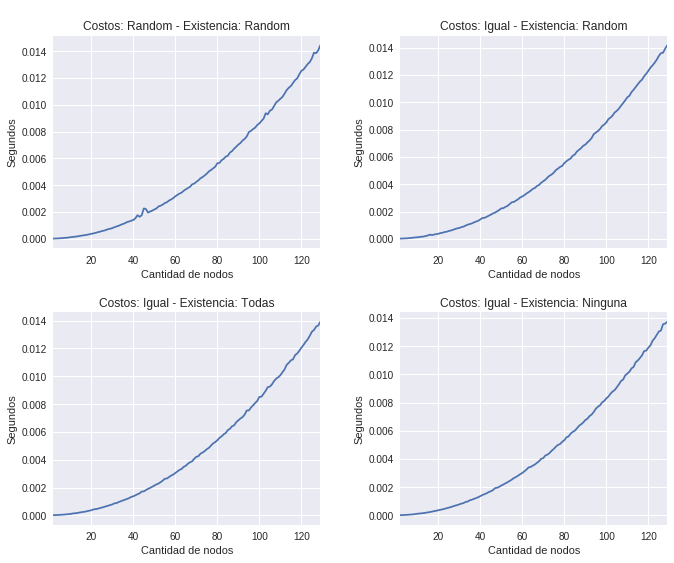
\includegraphics[width=0.9\textwidth]{imagenes/problema3/todos.png} \\
} 

Con estos resultados estamos bastante convencidos de lo que que sospechabamos: lo único que cambia el tiempo de cómputo del algoritmo es $n$. Para dar un cierre, hablemos un poco de cuando es que varía Prim, y veamos un poco que la pregunta inicial que teniamos tenía algún sentido. \\

Con otras implementaciones de Prim, en grafos poco densos es posible aprovechar el hecho de que no hayan tantos caminos para reducir el costo computacional. Sin embargo, como ya sabemos que nuestro grafo de entrada es completo, no hay mérito alguno en encarar el problema de esa forma, razón por la cual utilizamos matrices de adyacencias sin ningún otra estructura auxiliar en nuestro algoritmo. Como resultado, observemos que en nuestra implementación de Prim terminamos recorriendo la matriz entera un número constante de veces, en donde lo único que tiene injerencia es el tamaño de la matriz (el $n$).